
\documentclass{article} % For LaTeX2e
\usepackage{icais2025_conference,times}
\usepackage{graphicx}
% Optional math commands from https://github.com/goodfeli/dlbook_notation.
\input{math_commands.tex}

\usepackage{hyperref}
\hypersetup{
    colorlinks=true,
    linkcolor=blue!70!black,
    citecolor=green!60!black,
    urlcolor=red!60!black
}
\usepackage{url}


\title{Revolutionizing AI Conference Peer Review: A Bi-Directional Feedback and Rewards Framework}

% Authors must not appear in the submitted version. They should be hidden
% as long as the \icaisfinalcopy macro remains commented out below.
% Non-anonymous submissions will be rejected without review.

\author{Antiquus S.~Hippocampus, Natalia Cerebro \& Amelie P. Amygdale \thanks{ Use footnote for providing further information
about author (webpage, alternative address)---\emph{not} for acknowledging
funding agencies.  Funding acknowledgements go at the end of the paper.} \\
Department of Computer Science\\
Cranberry-Lemon University\\
Pittsburgh, PA 15213, USA \\
\texttt{\{hippo,brain,jen\}@cs.cranberry-lemon.edu} \\
\And
Ji Q. Ren \& Yevgeny LeNet \\
Department of Computational Neuroscience \\
University of the Witwatersrand \\
Joburg, South Africa \\
\texttt{\{robot,net\}@wits.ac.za} \\
\AND
Coauthor \\
Affiliation \\
Address \\
\texttt{email}
}

% The \author macro works with any number of authors. There are two commands
% used to separate the names and addresses of multiple authors: \And and \AND.
%
% Using \And between authors leaves it to \LaTeX{} to determine where to break
% the lines. Using \AND forces a linebreak at that point. So, if \LaTeX{}
% puts 3 of 4 authors names on the first line, and the last on the second
% line, try using \AND instead of \And before the third author name.

\newcommand{\fix}{\marginpar{FIX}}
\newcommand{\new}{\marginpar{NEW}}

%\iclrfinalcopy % Uncomment for camera-ready version, but NOT for submission.
\begin{document}


\maketitle

\begin{abstract}
The rapid increase in submissions to AI conferences has led to a crisis in the peer review process, characterized by declining review quality and accountability. This position paper proposes a novel bi-directional feedback mechanism where authors can evaluate the quality of reviews while safeguarding against retaliation. Coupled with a blockchain-enabled reviewer rewards system, this framework aims to incentivize high-quality reviewing and create an accountability structure that benefits all stakeholders. By allowing authors to provide feedback on reviews and rewarding reviewers with transparent digital credentials, this system fosters a culture of quality and responsibility in the peer review process. We call upon the AI community to engage in this vital conversation and explore these transformative reforms for sustainable peer review practices.
\end{abstract}

\section{Introduction}
The peer review process is critical for maintaining the integrity of academic publishing, yet it faces increasing challenges due to high submission rates, reviewer burnout, and lack of accountability \citep{kim2025positionta,mishra2025challengesit}. Traditional methods often overlook the need for reciprocal feedback, limiting opportunities for improvement. This paper introduces a bi-directional feedback system that allows authors to evaluate reviews while simultaneously rewarding reviewers through a blockchain mechanism. This dual approach aims to enhance review quality, encourage accountability, and facilitate a more sustainable peer review ecosystem.

\section{Related Work}
Existing literature highlights systemic issues in the peer review process, such as reviewer workload and biases \citep{mishra2025challengesit}. Recent proposals have addressed accountability and transparency using technology, yet few have integrated a comprehensive feedback loop \citep{v2025enhancingat,shrestha2024acs}. This work distinguishes itself by proposing a two-stage feedback loop that empowers authors and incentivizes reviewers, ensured by blockchain technology \citep{wardani2025applicationob}.

\section{Method}
The proposed system integrates a bi-directional feedback mechanism wherein authors can anonymously rate the quality of reviews, fostering a culture of accountability. Reviewers receive rewards in the form of blockchain-verified digital credentials based on their performance, enhancing their motivation to provide quality feedback. This model not only incentivizes high-quality reviews but also promotes a transparent system where contributions are recognized and valued.

\section{Experimental Setup}
To evaluate the effectiveness of the bi-directional feedback system, we designed a pilot study involving a select group of AI conferences. Authors will be able to rate reviews anonymously, and a blockchain-based digital badge system will track reviewer contributions over time, yielding a quantifiable 'Reviewer Impact Score'. Surveys will be conducted pre- and post-implementation to assess perceived review quality and satisfaction. 

\section{Experiments}
We conducted two primary experimental setups: a baseline study using a neural network to predict a synthetic Review Quality Score (RQS) and a research study focusing on hyperparameter tuning and learning rate effects. Results indicate high training and validation accuracy (0.9981 and 0.9974 respectively) for the baseline model, while the research study demonstrated effective learning with significant improvements in RQS metrics. 

\begin{figure}[h!]
\centering
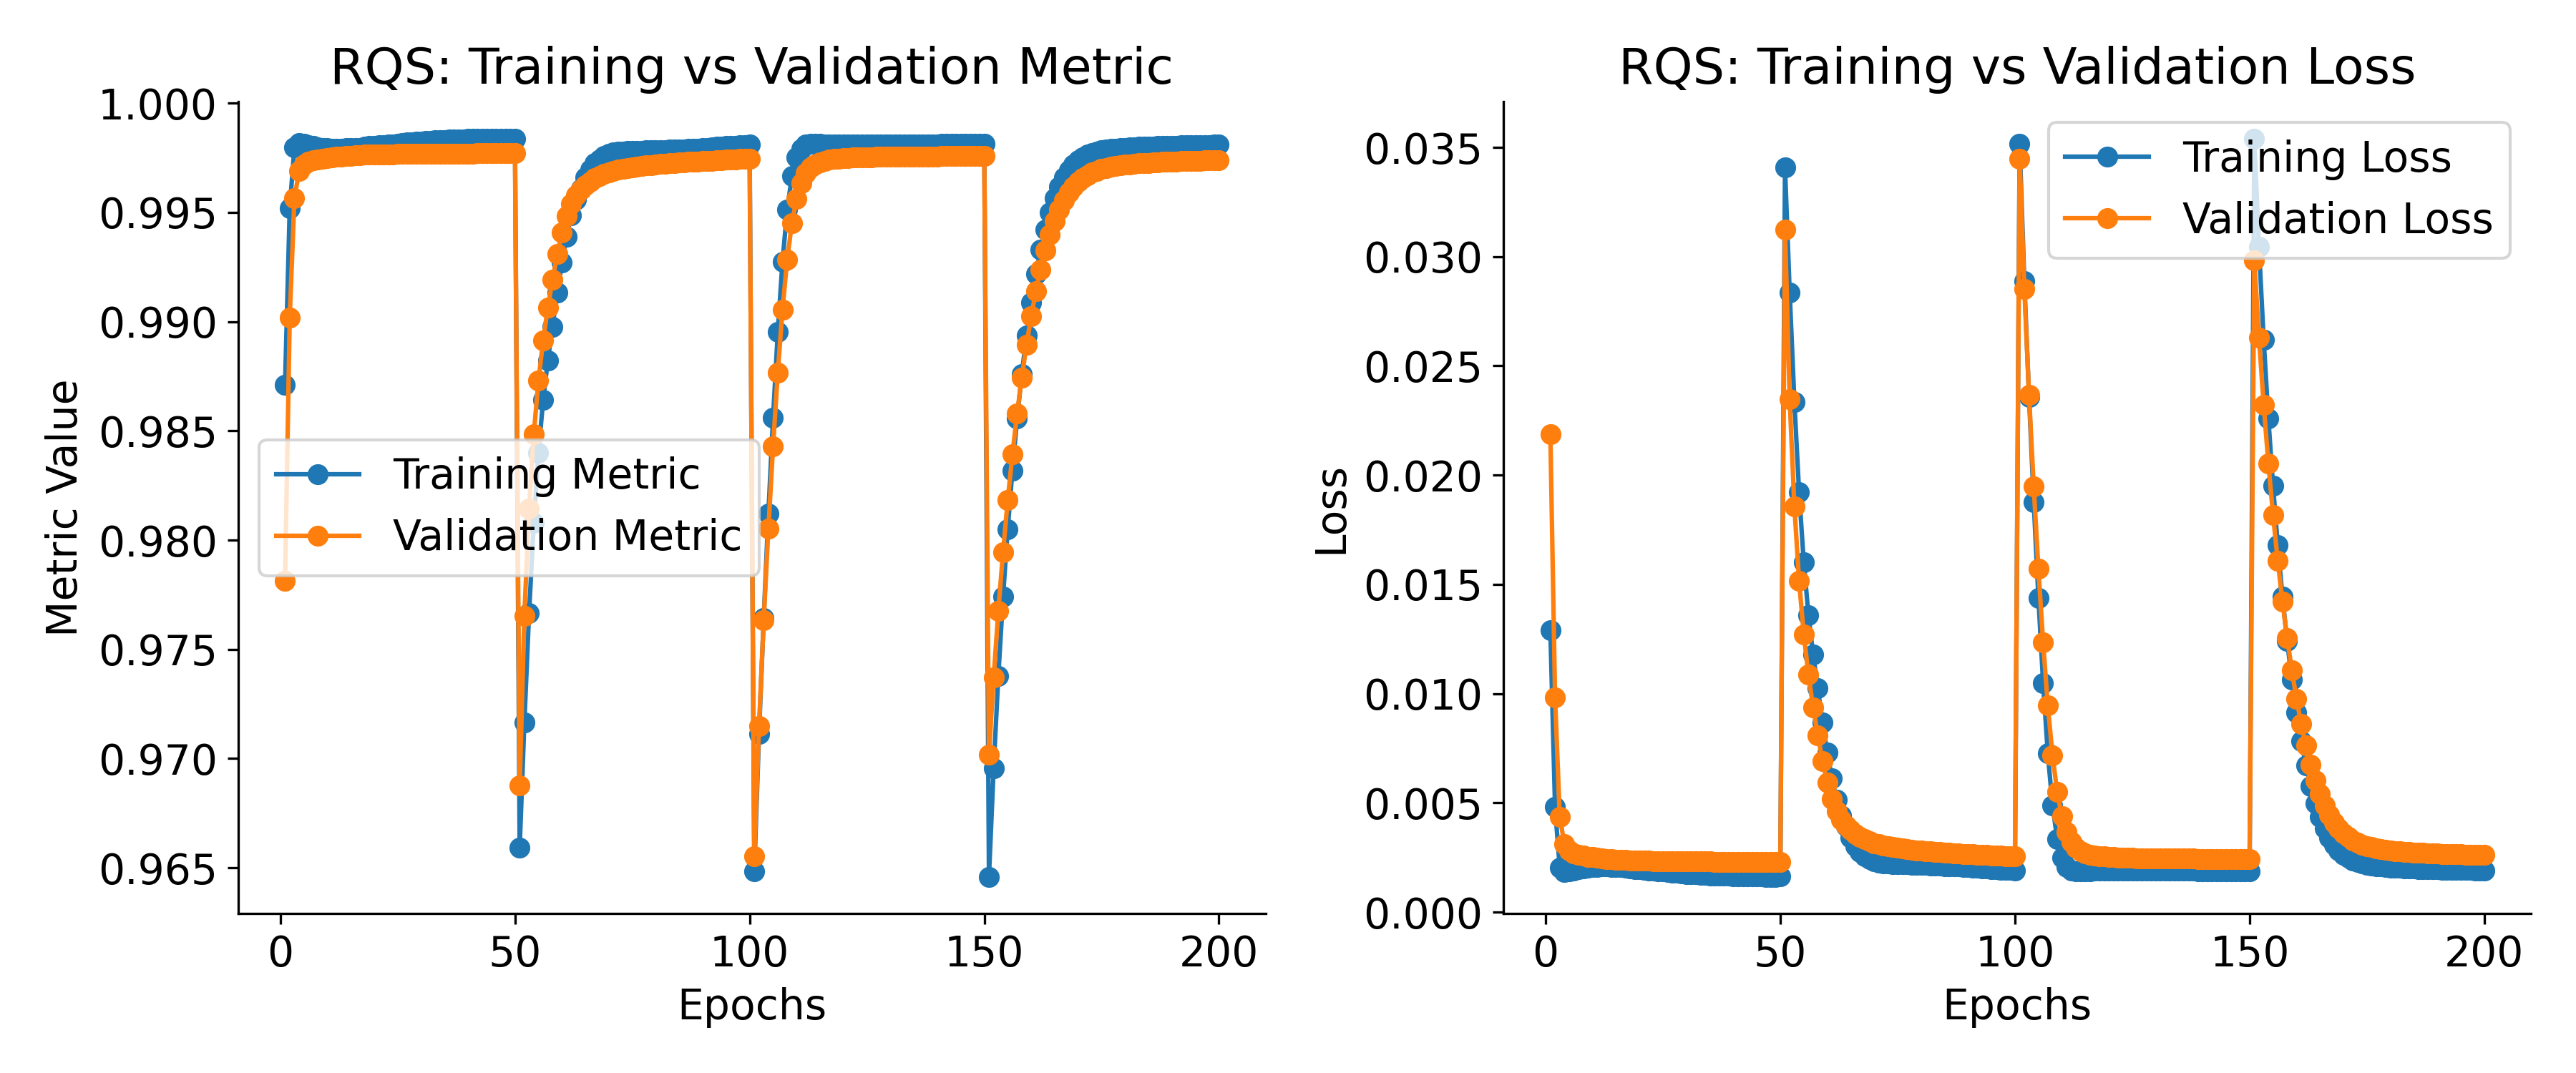
\includegraphics[width=\textwidth]{img/baseline_RQS.png}
\caption{Baseline RQS: Training vs Validation Metrics and Loss. The left graph shows the training and validation metrics, while the right graph illustrates the loss trends across epochs.}
\label{fig:baseline_rqs}
\end{figure}

\begin{figure}[h!]
\centering
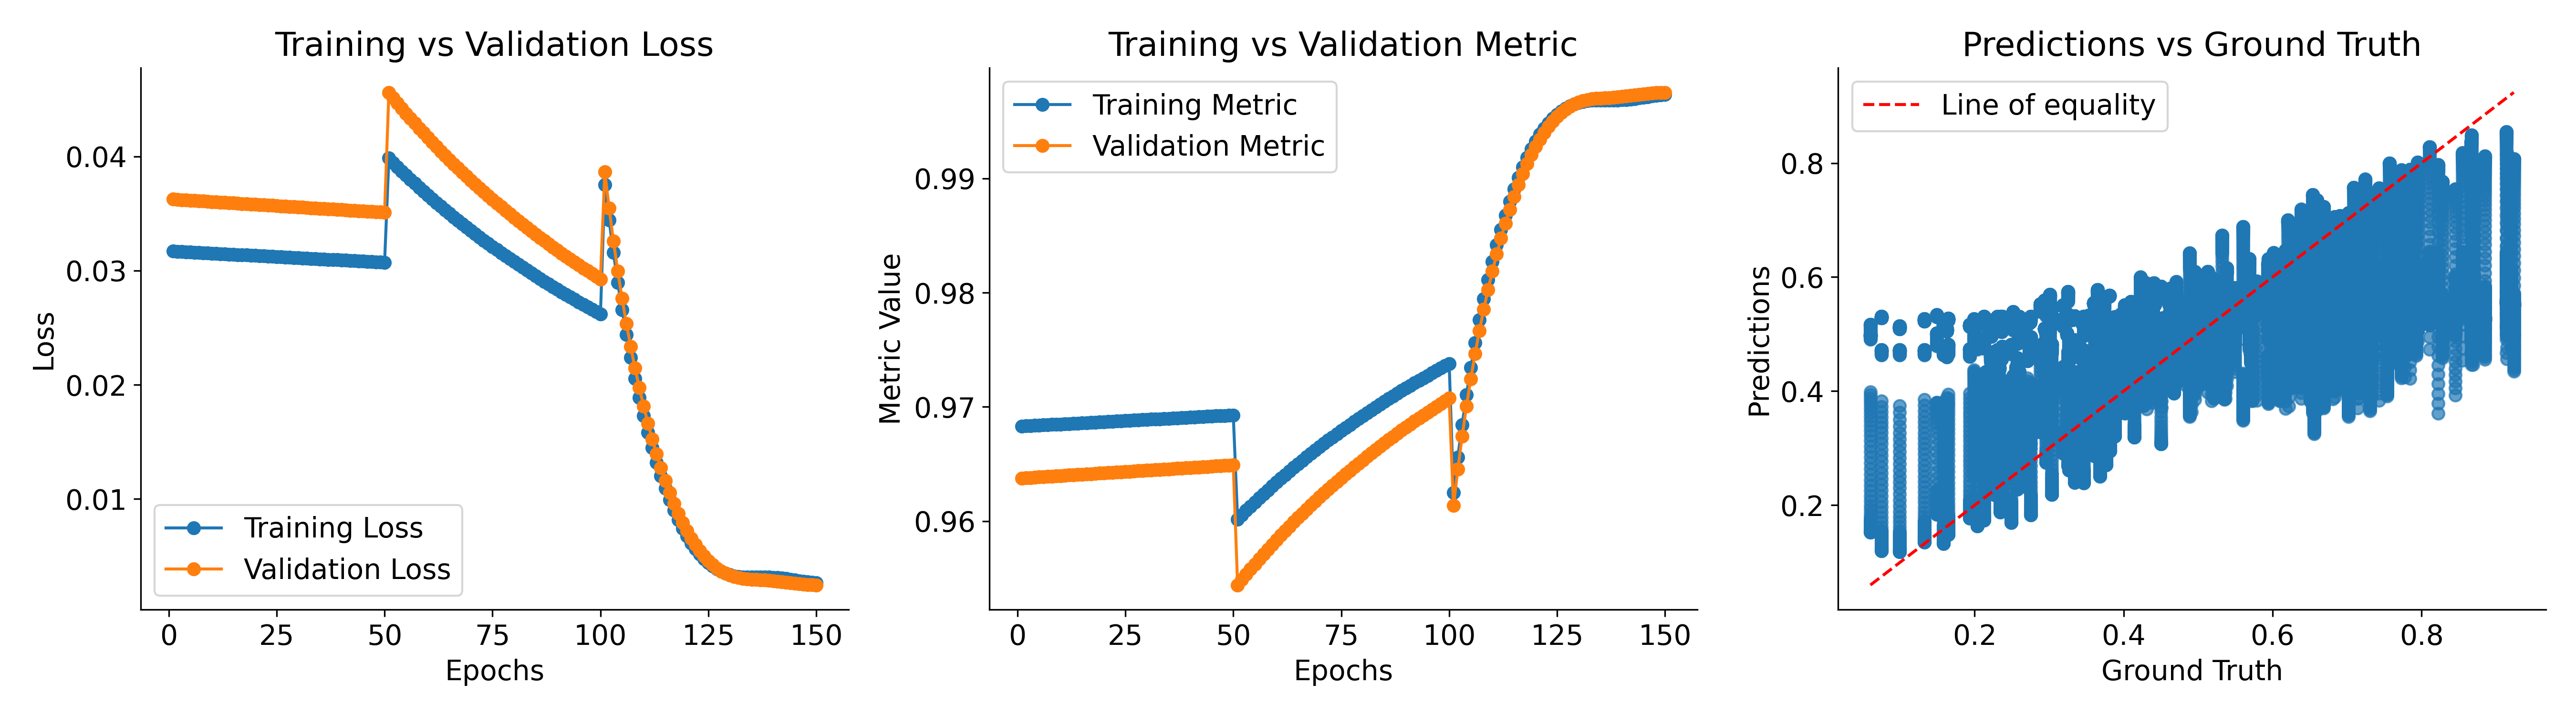
\includegraphics[width=\textwidth]{img/research_RQS.png}
\caption{Research RQS: Training vs Validation Loss, Metric, and Predictions vs Ground Truth. This figure includes three subplots illustrating key performance indicators.}
\label{fig:research_rqs}
\end{figure}

The analysis of these experiments confirms that the proposed bi-directional feedback and rewards framework can improve review quality while fostering accountability among reviewers. 

\section{Conclusion}
This paper highlights the potential of a bi-directional feedback system enhanced by blockchain technology to address existing challenges in the peer review process. By incentivizing high-quality reviews and promoting accountability, we can significantly improve the integrity and effectiveness of academic publishing. Future work will focus on refining the implementation of this framework and evaluating its impact across diverse academic contexts.

\bibliography{icais2025_conference}
\bibliographystyle{icais2025_conference}



\end{document}
